\section{Experimentos}
\label{sec:experiments}

Para cada experimento se estudian cinco algoritmos:
una implementaci\'on base de \astar que sirve de referencia,
una implementaci\'on de caminos simples aleatorios mediante
b\'usqueda en profundidad, \ambush, \pambush con mecanismo
de prioridad determinado por la distancia real de los agentes
a la meta y finalmente, \sarambush.

presentan resultados del incremento medio porcentual de los caminos.
Para cada topolog\'ia de grafo, se generan aleatoriamente 100 grafos,
sobre los cuales se ejecutan experimentos con 100 disposiciones distintas
de agentes y del nodo objetivo.
Para cada uno de estos algoritmos se muestra el valor de emboscada
utilizando la m\'etrica originalmente propuesta y utilizando la
m\'etrica propuesta en el presente trabajo. El n\'umero de agentes
es variado con el fin de mostrar su impacto en el grado de emboscada
y en el incremento derivado de la escogencia de caminos sub\'optimos.
Adem\'as se muestran resultados con las dos instancias de mapas ($g1$ y $g2$)
presentadas en el trabajo previo \cite{FGC12} con 60 y 85 nodos
respectivamente. Estos mapas provienen de la poligonalizaci\'on del mapa
de juego en pol\'igonos. Estas restricciones son ampliamente utilizadas
en juegos\cite{MF09}. Estos grafos se pueden visualizar en la figura \ref{fig:gs}.

\begin{figure}[htb]
	\begin{center}
		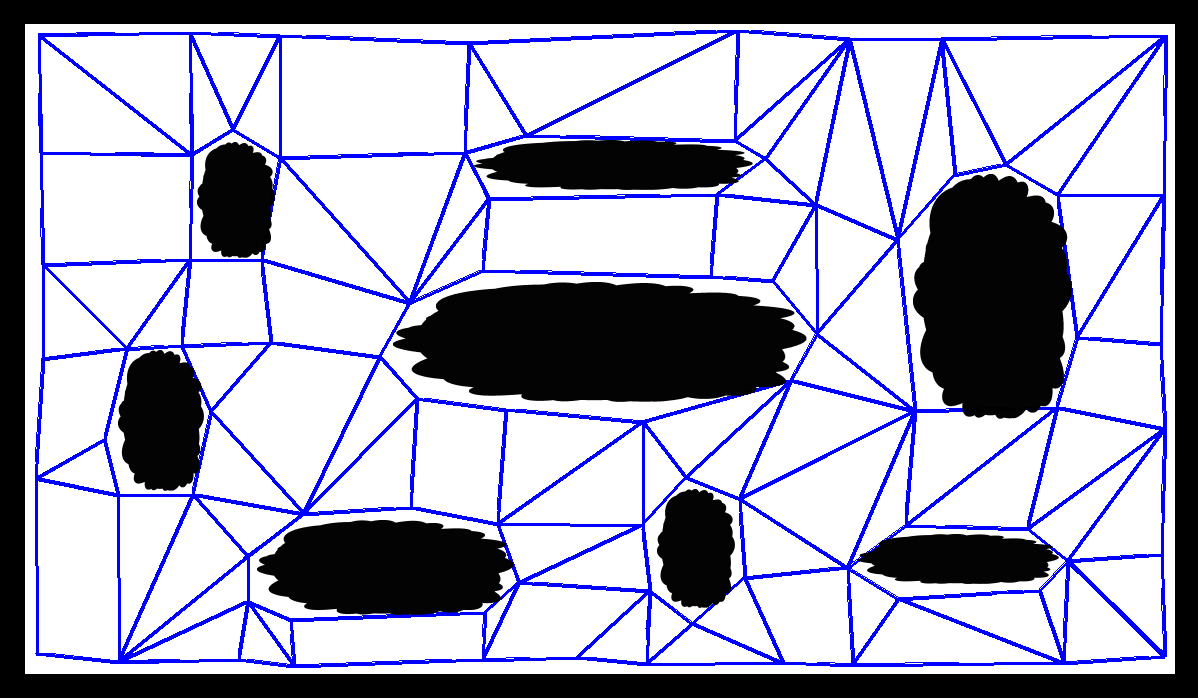
\includegraphics[scale=0.23]{figures/g1.png}
		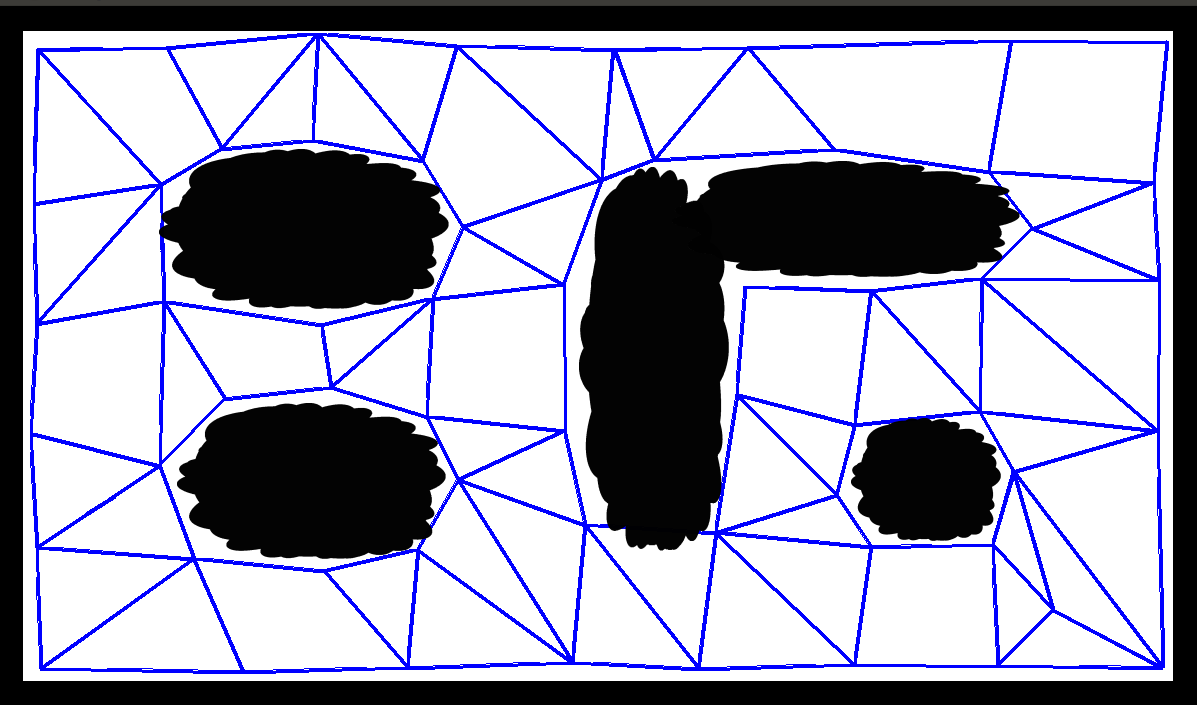
\includegraphics[scale=0.23]{figures/g2.png}
	\end{center}
	\caption{\label{fig:gs}
	     \textbf{Arriba:} Mapa 1 poligonalizado (60 pol\'igonos).
	     \textbf{Abajo:} Mapa 2 poligonalizado (85 pol\'igonos).
     }
\end{figure}
